\section{Experimentation}
%Describe experiments and performance measures
%Two measures of interest, time to solution and quality of solutions
We conduct a series of experiments for the noiseless and noisy simulations of our algorithm in this section. We empirically compare against the \comment[id=jlt]{Need referencing either the actual papers, or just saying the acronyms earlier}IAE and MLAE algorithms. As the update steps for these algorithms are equivalent to sampling from a Bernoulli distribution for a given choice of $\theta_0$ and noise level we sample directly from the Bernoulli distribution instead of simulating the dynamics of a quantum system for each algorithm. This algorithm has also been implemented and tested using Qiskit \cite{Qiskit}, with a view for future experiments with quantum simulators and quantum hardware.


\subsection{Simulation}
\subsubsection{Noiseless}
First, we explore the convergence time for $\theta \in [0, \pi/2]$. As shown in \cite{callison_2022_amp_with_jitter}, so-called exceptional points with poor convergence occur near to rational multiples of $\pi$, therefore we sample values of $\theta$ from continuous distributions instead of equally spaced angles. Figure \ref{fig::ExAE-converge-quarter-circle} shows that the convergence for $\theta$ close to $0$ is several orders of magnitude larger than convergence for other values. For this reason, we consider partitioning the space $\Theta = [0, \pi/2]$ into the central region $\Theta_0 = [\frac{\pi}{12}, \frac{5 \pi}{12}]$ and the edge region $\Theta_1 = \Theta \setminus \Theta_0 = [0, \frac{\pi}{12})$. This is region of poor convergence is inherent to the use of likelihood-based sampling regimes, and is not shared by IAE (see \ref{fig::Iae-converge-quarter-circle}).

\begin{figure}[htbp]
	\centering

	\begin{subfigure}{0.45\textwidth}
		\centering
		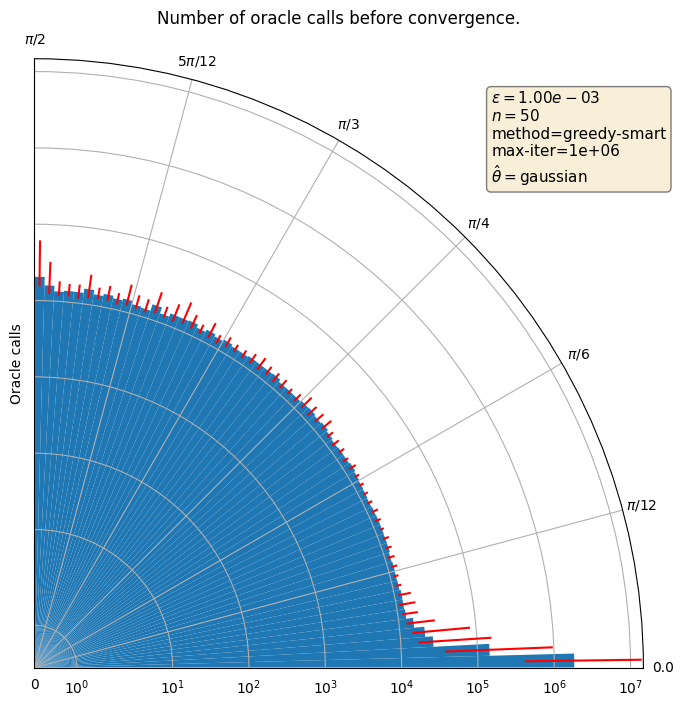
\includegraphics[width=\linewidth]{ExAE-converge-quarter-circle}
		\caption{Median number of oracle calls for SAE to converge to a precision of $\varepsilon = 10^{-3}$, with 25\% and 75\% quartiles shown. Each bar is a region of width $\pi / 120$ with the median number of oracle calls calculated from 50 values of true value $\theta_0$ selected uniformly at random. The prior for each iteration is taken to be $N(\tilde{\theta}_0, 1)$, where $\tilde{\theta}_0$ is sampled from a $N(\theta_0, 0.1)$ distribution and success probability $1 - \alpha$ with $\alpha = 0.01$.}
		\label{fig::ExAE-converge-quarter-circle}
	\end{subfigure}
	\hfill
	\begin{subfigure}{0.45\textwidth}
		\centering
		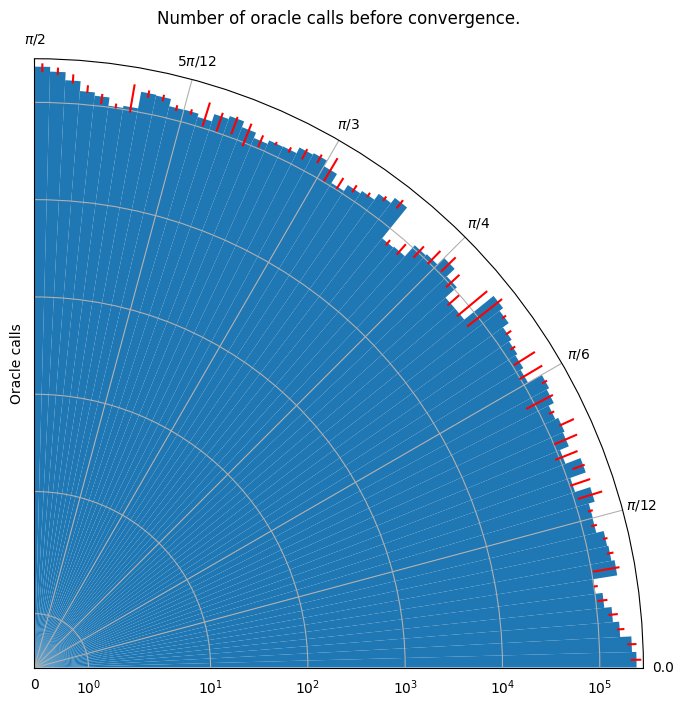
\includegraphics[width=\linewidth]{Iae-converge-quarter-circle}
		\caption{Median number of oracle calls for IAE to converge to a precision of $\varepsilon = 10^{-3}$, with 25\% and 75\% quartiles shown. Each bar is a region of width $\pi / 120$ with the median number of oracle calls calculated from 50 values of true value $\theta_0$ selected uniformly at random, and a success probability $1 - \alpha$ with $\alpha = 0.01$}
		\label{fig::Iae-converge-quarter-circle}
	\end{subfigure}
\end{figure}
\comment[id=cdv]{Misses a caption of the 'full' figure.}
\comment[id=cdv]{It's actually from 1000 values. I can change that either in the figure, or in the caption.}
\begin{center}
	\color{red}
	(The following is all conjecture as we don't have a comparison graph.) \\
As seen in Figure \ref{fig::ExAE-converge-on-theta1}, the set $\Theta_1$ performs poorly for all methods that take a statistical approach. This region contains points where the variance reduction factor approaches 0, with the extreme points where $\theta= 0, \pi$.
\end{center}

\begin{figure}[htbp]
	\centering
	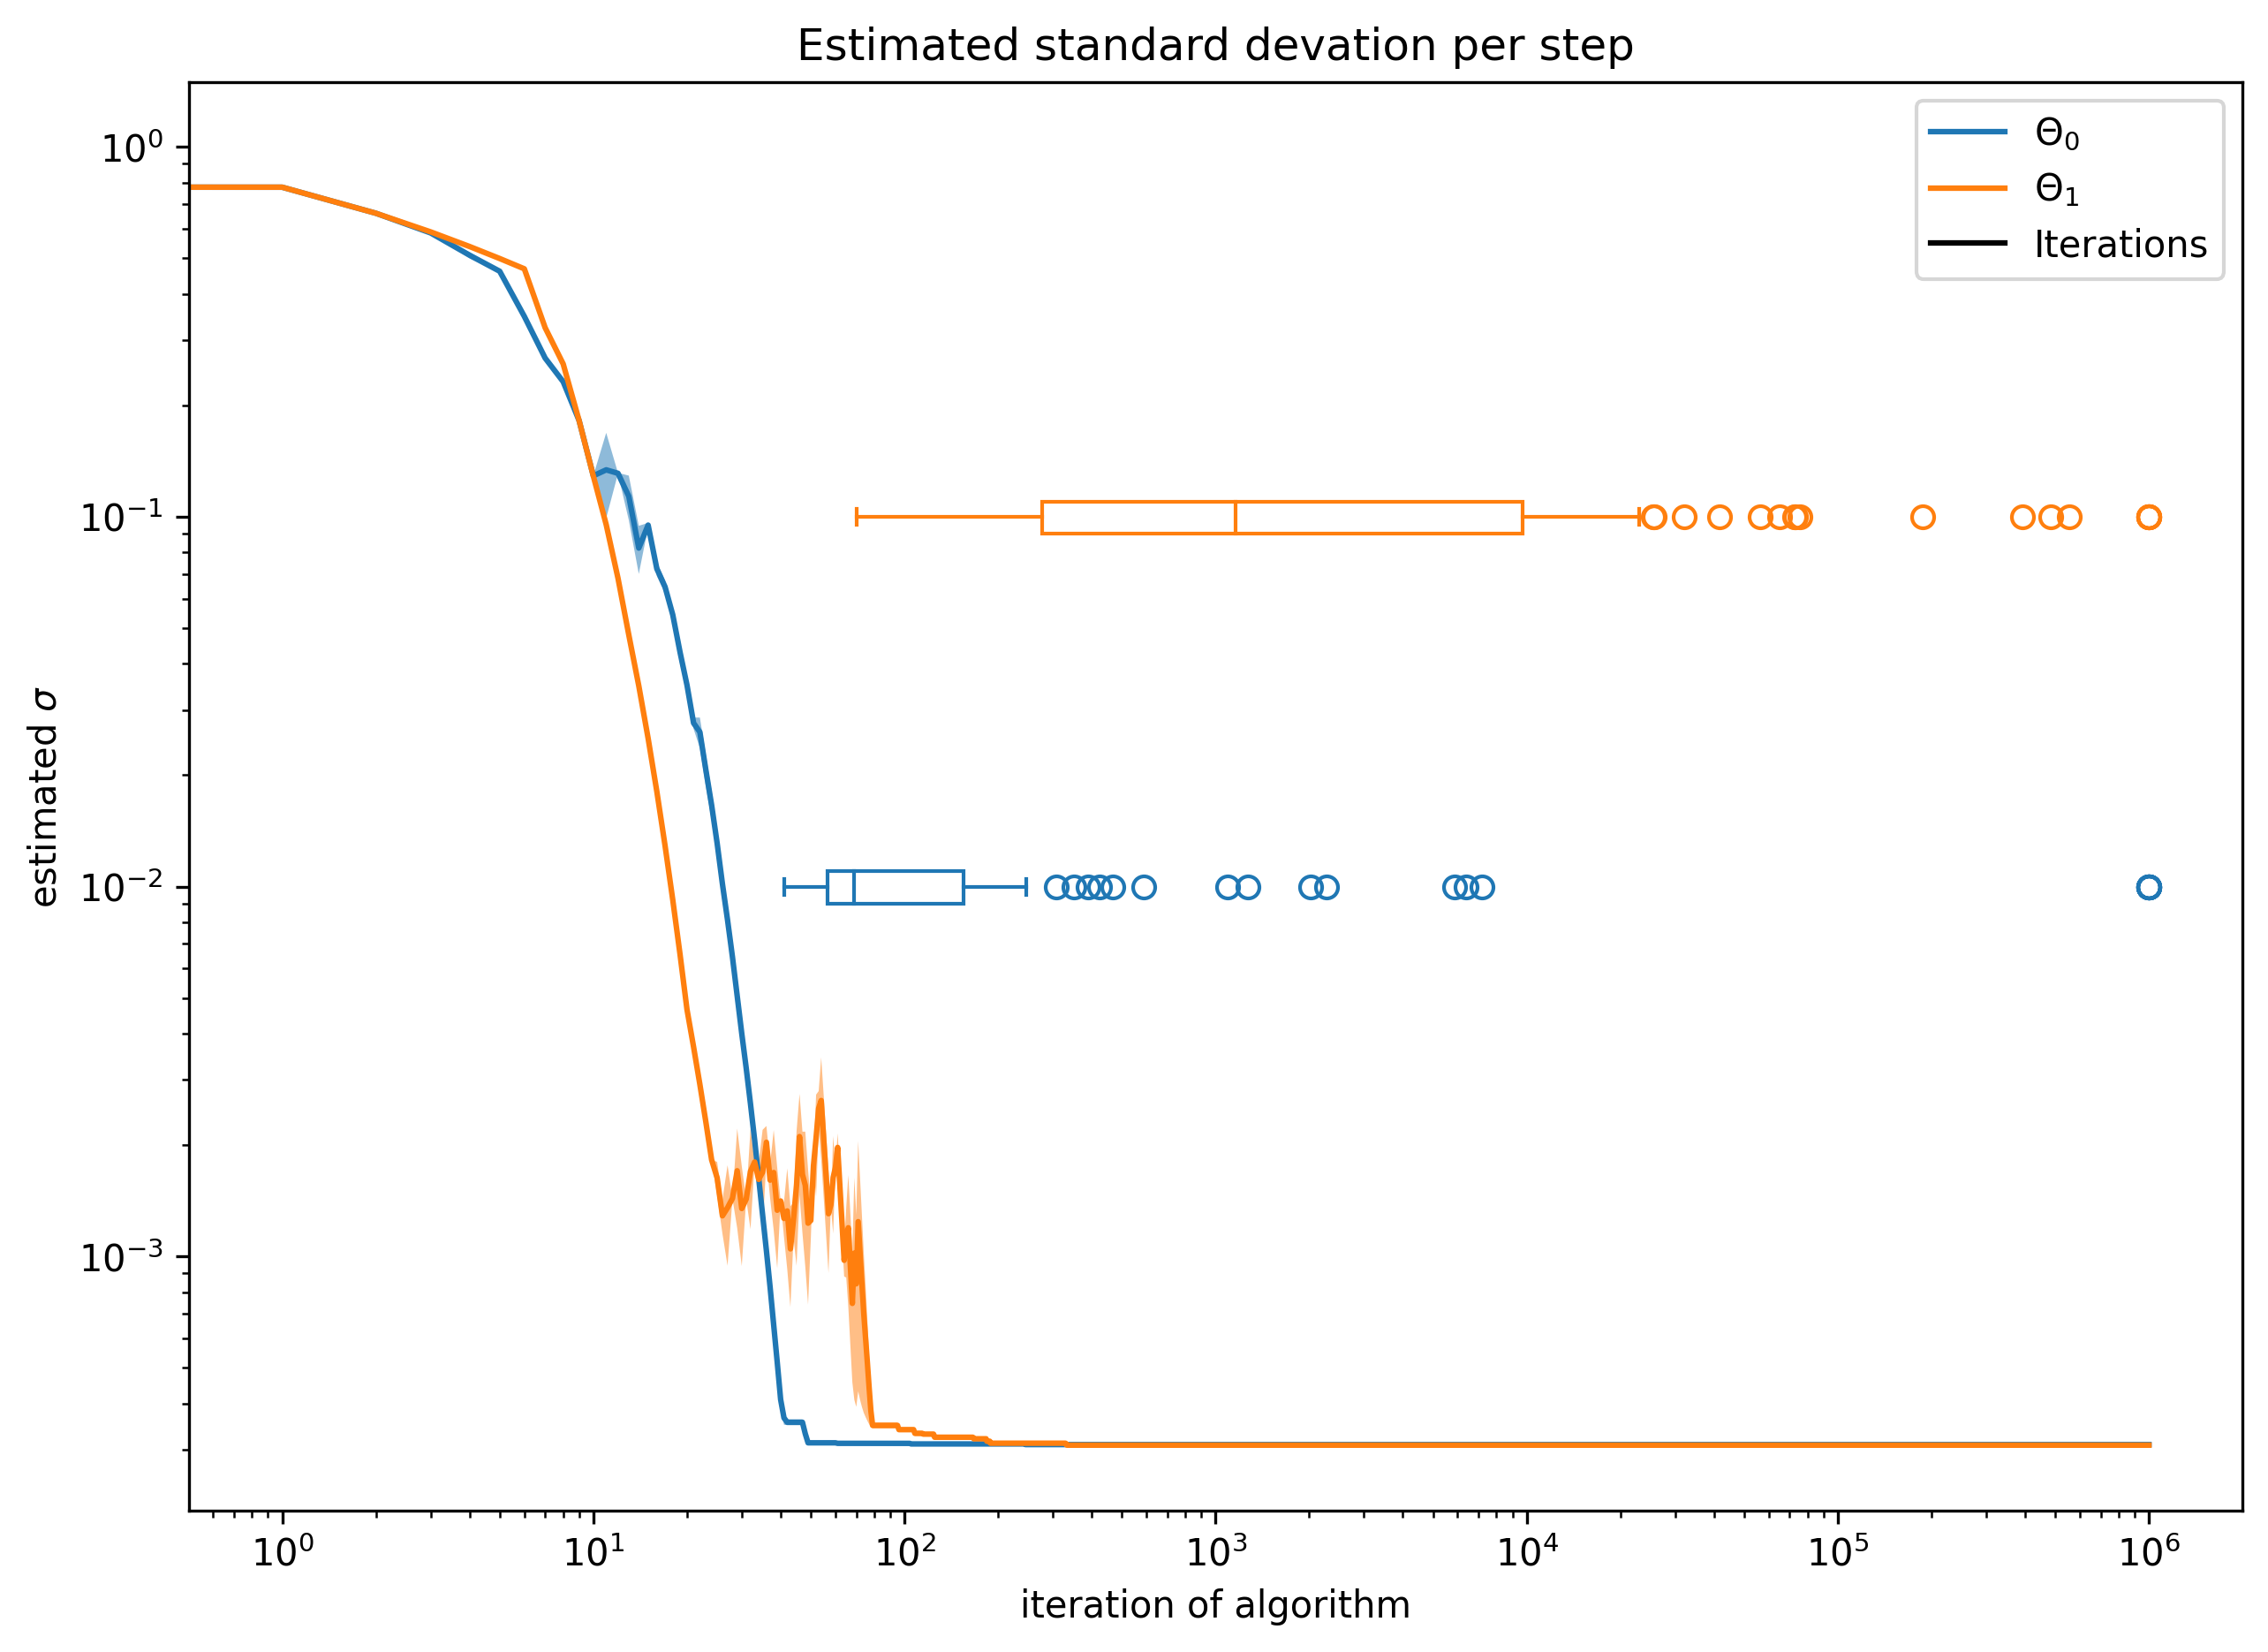
\includegraphics[scale=0.3]{ExAE-std-per-step}
	\caption{Median standard deviation for fixed error rate $\varepsilon = 10^{-3}$ against time step for $\theta_0 \in \Theta_0$ and $\theta_0 \in \Theta_1$. We sample $\theta_0$ from a uniform distribution of $x$ and $50$ samples for $\Theta_0$ and $ \Theta_1$ respectively. The prior for each iteration is taken to be $N(\theta_0, 1)$ and success probability $1 - \alpha$ with $\alpha = 0.01$. The box plots show the Q1, Q2 and Q3 algorithm termination times for the recorded runs.}
	\label{fig::ExAE-std-per-step}
\end{figure}

\begin{figure}[htbp]
	\centering
	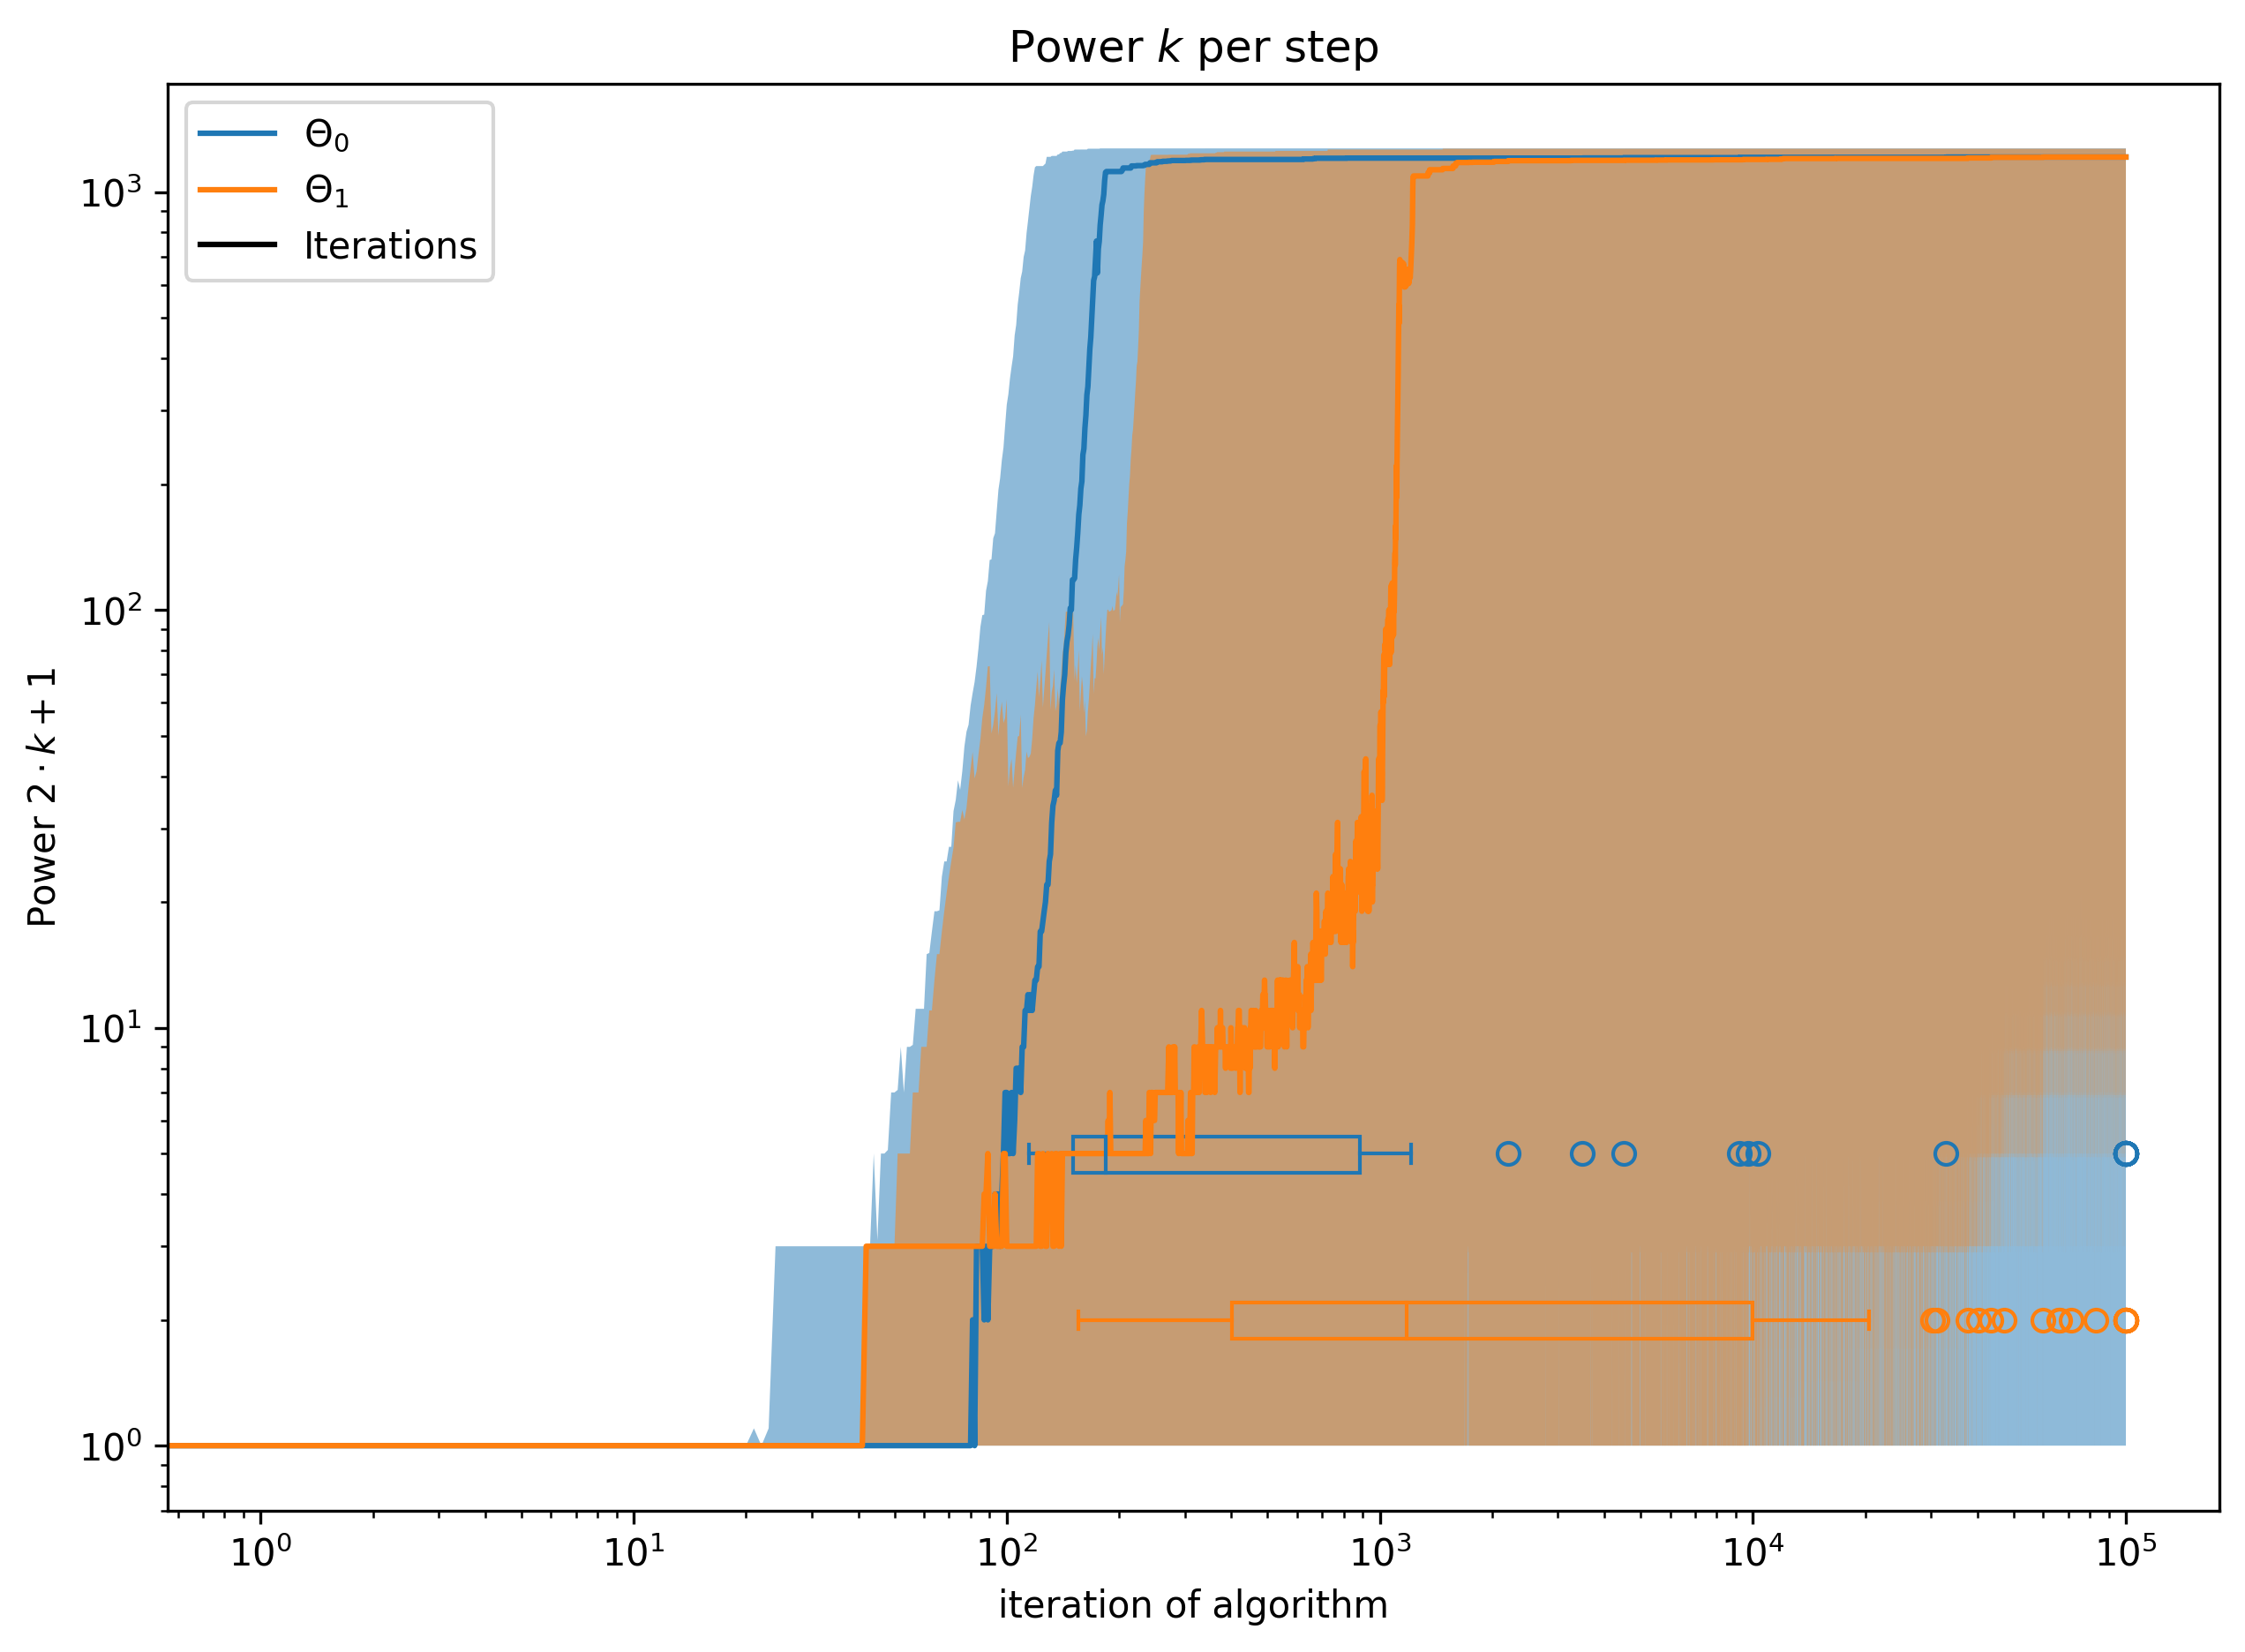
\includegraphics[scale=0.3]{ExAE-depth-per-step}
	\caption{Median depth for fixed error rate $\varepsilon = 10^{-3}$ against time step for $\theta_0 \in \Theta_0$ and $\theta_0 \in \Theta_1$. We sample $\theta_0$ from a uniform distribution of $x$ and $50$ samples for $\Theta_0$ and $ \Theta_1$ respectively. The prior for each iteration is taken to be $N(\theta_0, 1)$ and success probability $1 - \alpha$ with $\alpha = 0.01$. The box plots show the Q1, Q2 and Q3 algorithm termination times for the recorded runs.}
	\label{fig::ExAE-depth-per-step}
\end{figure}

From now on, we restrict to considering $\theta \in \Theta_0$.

A source of potential error in this algorithm is the normal approximation made at each step, which removes the theoretical guarantees of the \comment[id=jlt]{This may need references to earlier in the algorithm section}Bernstein-von-Mises theorem. This can be seen in Figure \ref{fig::ExAE-actual-prec-vs-expected-prec}, where should expect $(1-\alpha)\%$ of the points to lie above the diagonal. As a mitigation technique, we post-process the measurement data using the MLE estimator, and recover some of the desired accuracy.

\begin{figure}[htbp]
	\centering
	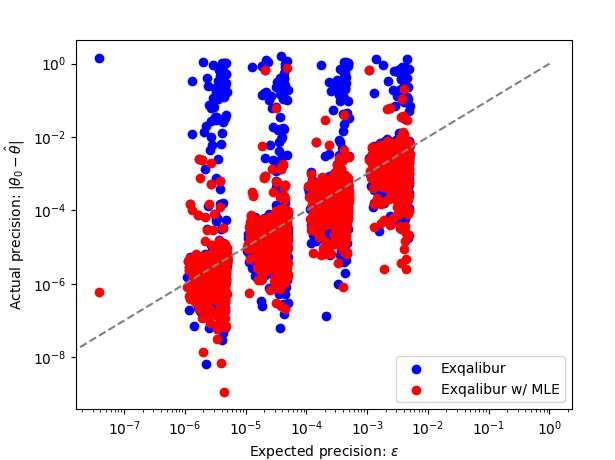
\includegraphics[scale=0.3]{ExAE-actual-prec-vs-expected-prec}
	\caption{Actual precision of the final estimate for SAE with and without MLE post-processing. We sample $\theta_0 \in \Theta_0$ from a uniform distribution of $x$ and $50$ for target precisions of $\varepsilon = 10^{-3}, 10^{-4}, \ldots, 10^{-7} $. The prior for each iteration is taken to be $N(\theta_0, 1)$ and success probability $1 - \alpha$ with $\alpha = 0.01$.}
	\label{fig::ExAE-actual-prec-vs-expected-prec}
\end{figure}

\begin{figure}[htbp]
	\centering
	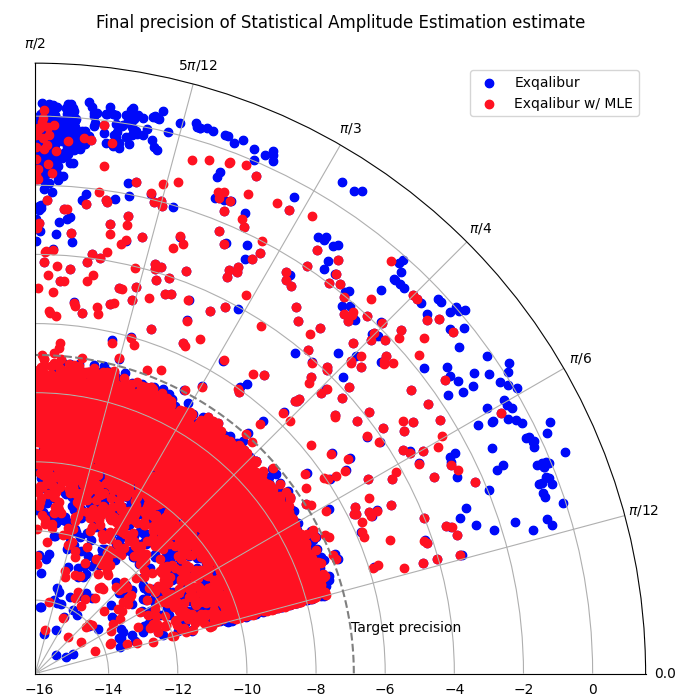
\includegraphics[scale=0.2]{ExAE-actual-prec-over-theta}
	\caption{Actual precision of the final estimate for SAE with and without MLE post-processing. We sample $\theta_0 \in \Theta_0$ from a uniform distribution of $x$ and $500$ for a target precision of $\varepsilon = 10^{-3}$. The prior for each iteration is taken to be $N(\theta_0, 1)$ and success probability $1 - \alpha$ with $\alpha = 0.01$.}
	\label{fig::ExAE-actual-prec-over-theta}
\end{figure}

We compare the performance of SAE to IAE and MLAE, and observe that in the noiseless case we achieve similar numbers of oracle queries to IAE. However, there still remain some points for which SAE fails to satisfactorily converge.

\begin{figure}[htbp]
	\centering
	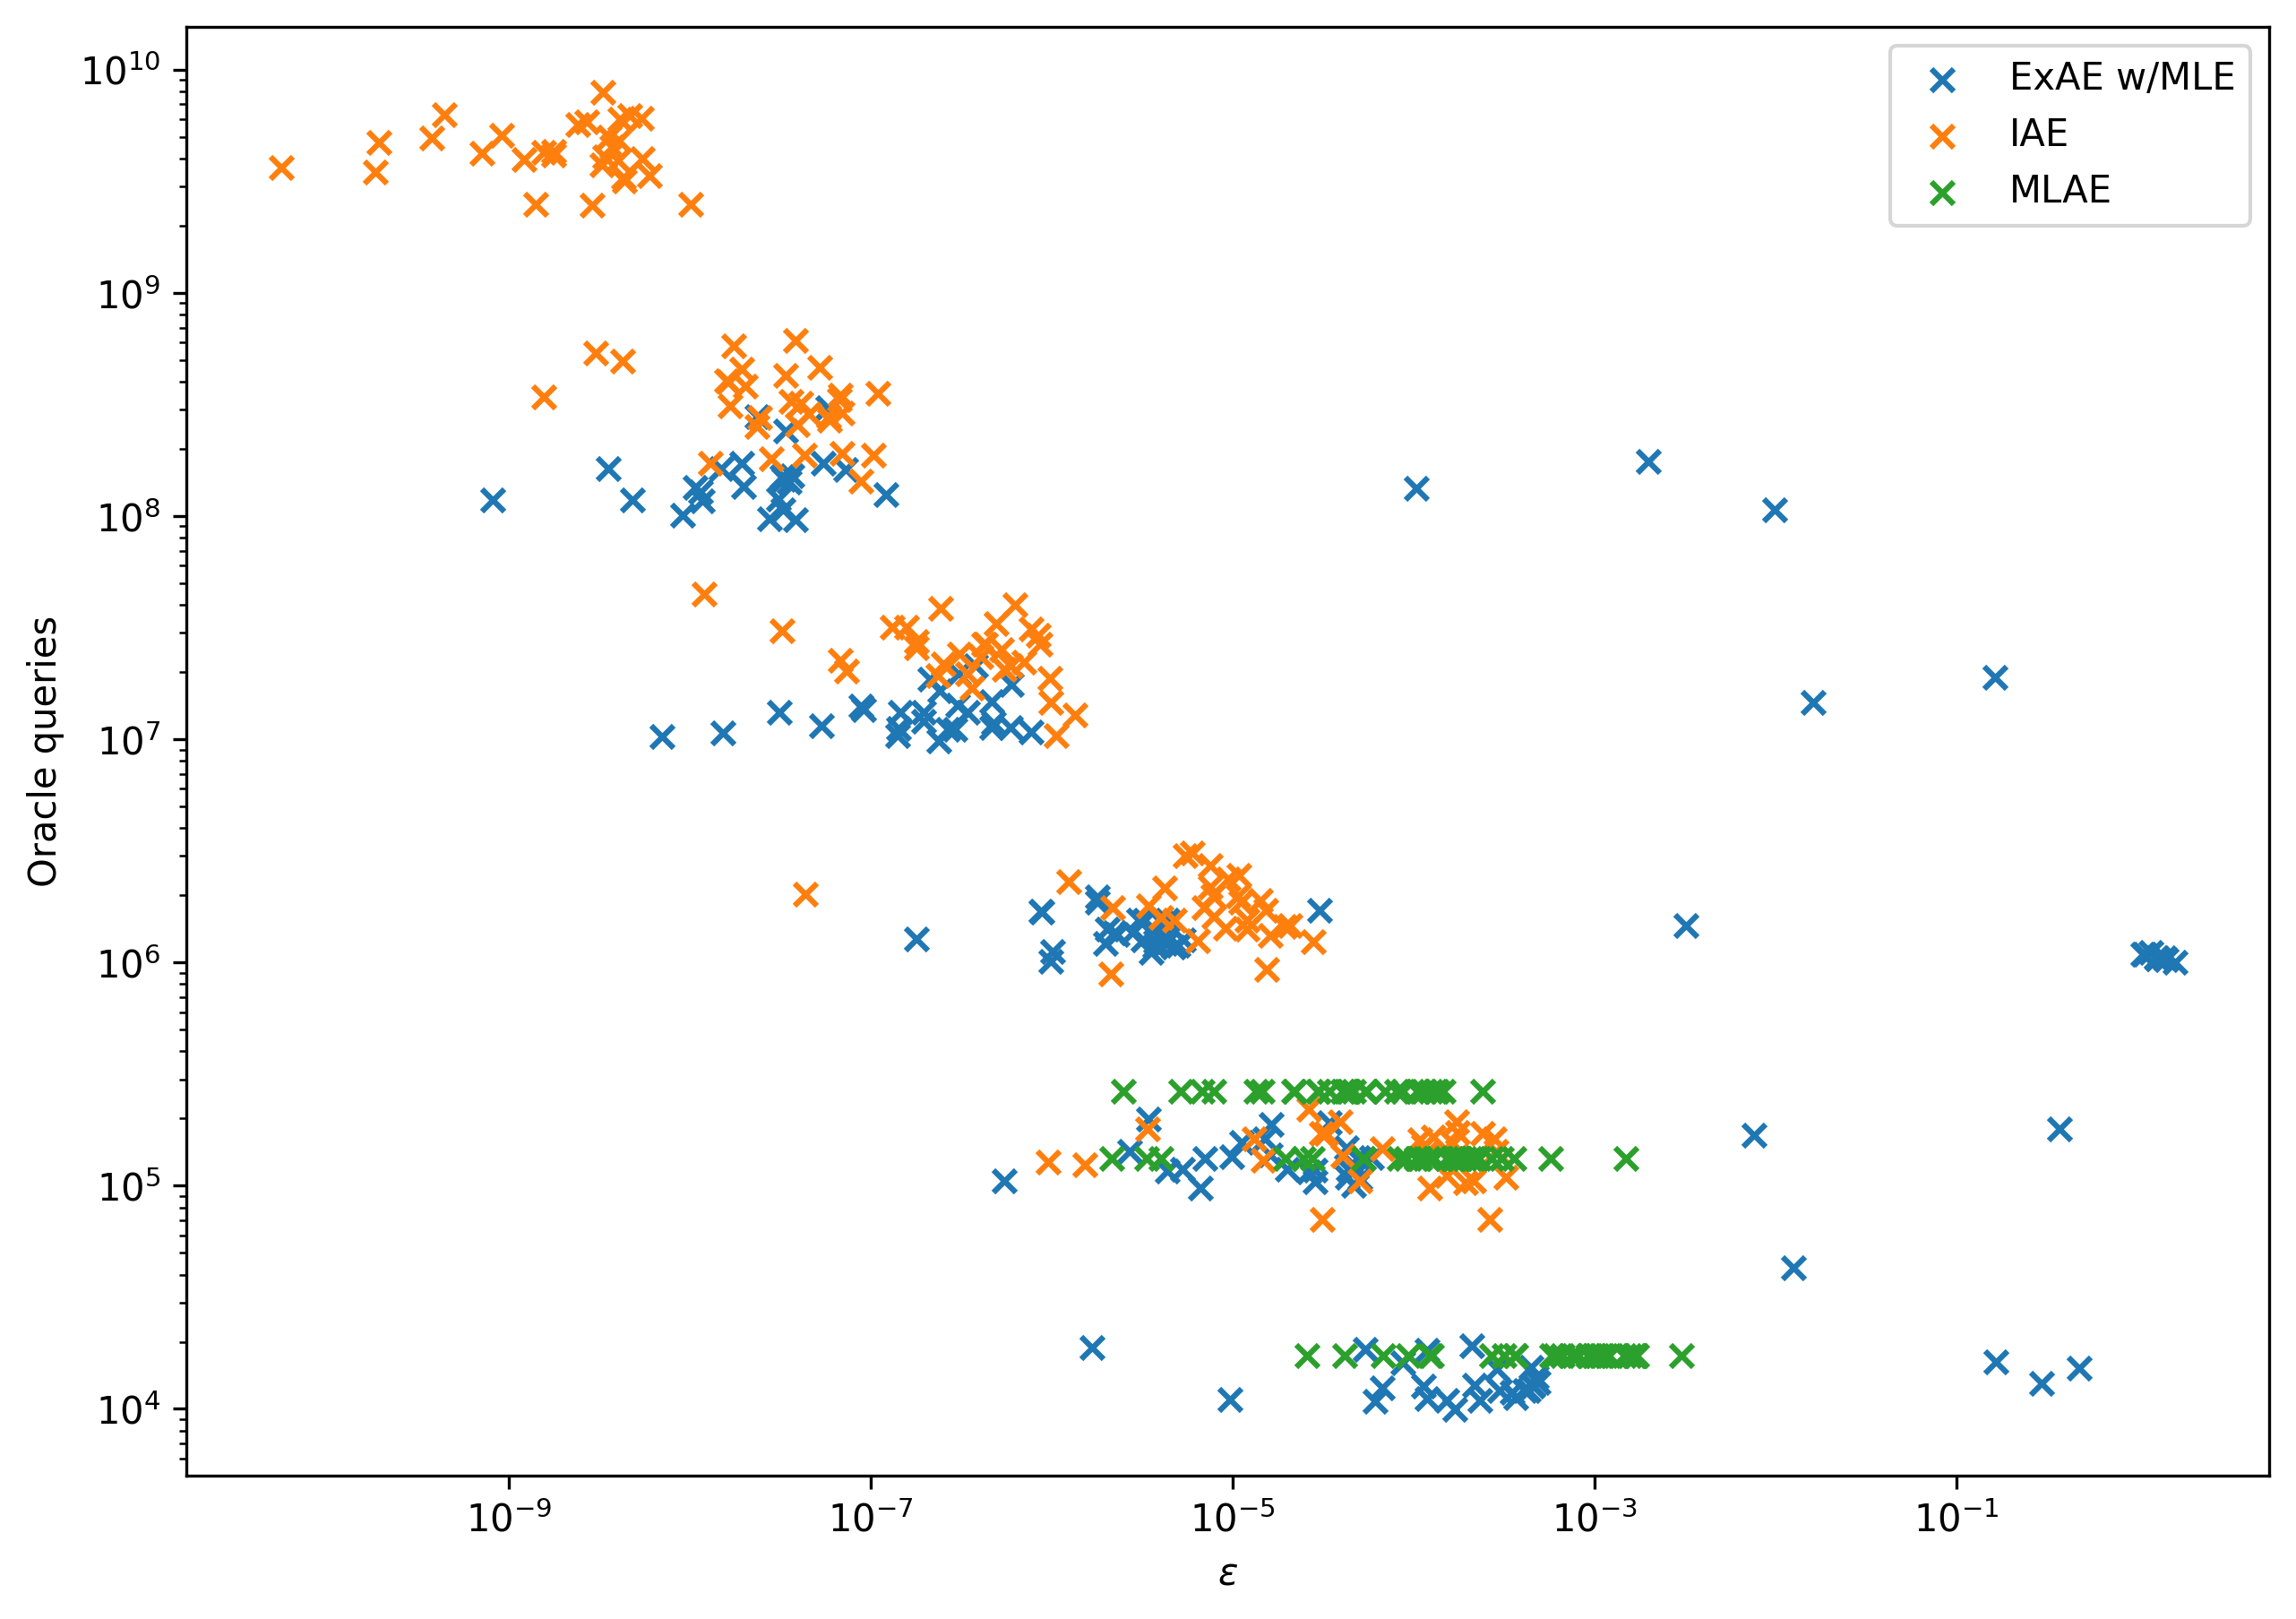
\includegraphics[scale=0.5]{query-comparison-noiseless}
	\caption{Actual precision versus total number of oracle queries used for IAE, MLAE and SAE. We target precisions of $\varepsilon = 10^{-3}, 10^{-4}, \ldots , 10^{-7}$, with each point a single value of $\theta_0 \in \Theta_0$ and take the final precision to be half the width of the confidence interval. We sample uniformly from $\Theta_0$ for 30 values of $\theta_0$. Each value of $\theta_0$ is evaluated for all algorithms and each target $\varepsilon$. The prior for each iteration is taken to be $N(\theta_0, 1)$ and success probability $1 - \alpha$ with $\alpha = 0.01$.}
	\label{fig::query-comparison-noiseless}
\end{figure}


\begin{figure}[htbp]
	\centering
	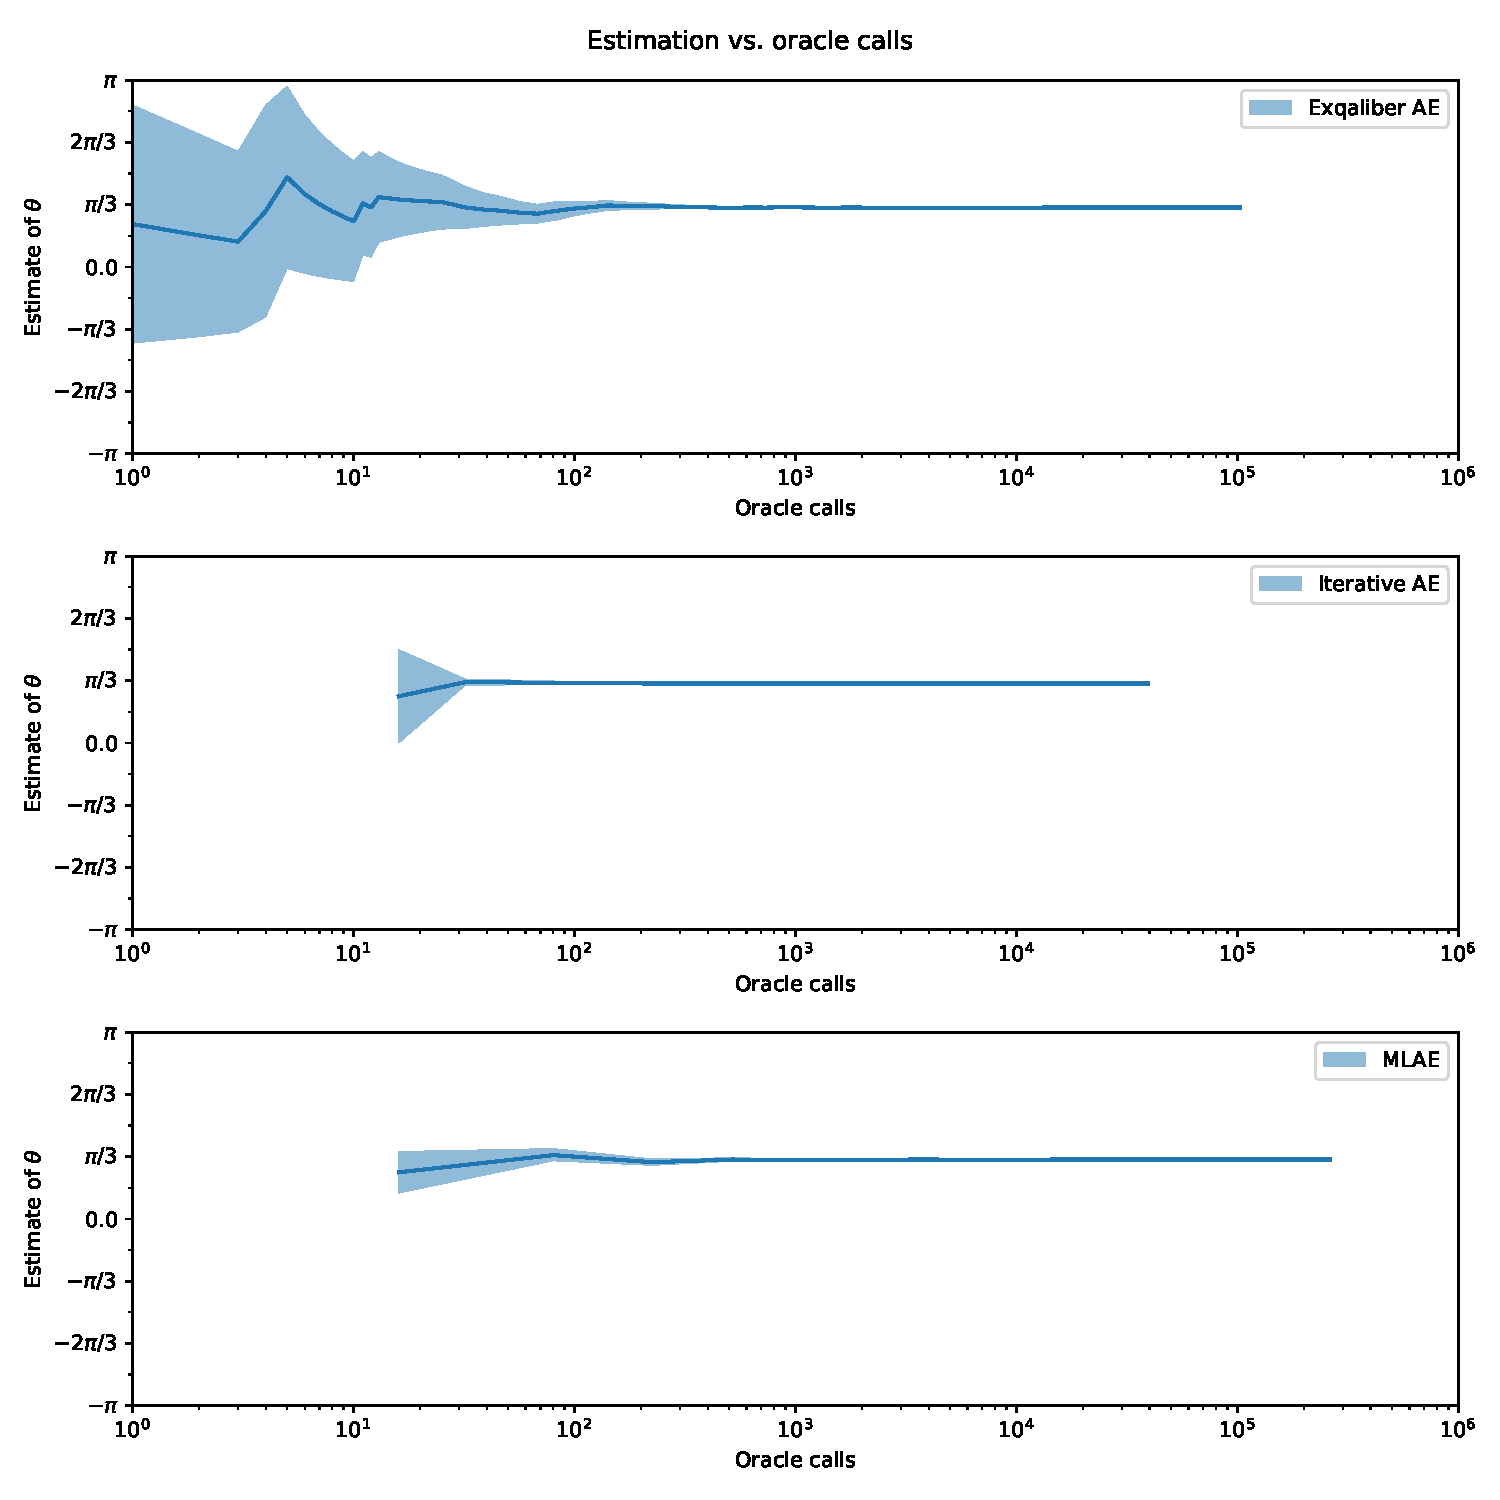
\includegraphics[scale=0.3]{compare-paths-oracle-calls}
	\caption{Confidence intervals for a single run of SAE, IAE and MLAE with $\theta_0 = 1$. The prior for SAE is taken to be $N(\pi/2, 1)$ and success probability $1 - \alpha$ with $\alpha = 0.01$. As IAE and MLAE use a fixed number of shots per step, the number of oracle calls does not start at 0.}
	\label{fig::compare-paths-oracle-calls}
\end{figure}

For the SAE routine, we also calculate the expected and exact probability of the Bernoulli sample at each stage. \ref{fig::exae-expected-probability} is a typical example of a SAE run, where the probability is initially expected to be 0 for a substantial amount of time, before approaching $\frac{1}{2}$ for the remainder of the run.

\begin{figure}[htpb]
	\centering
	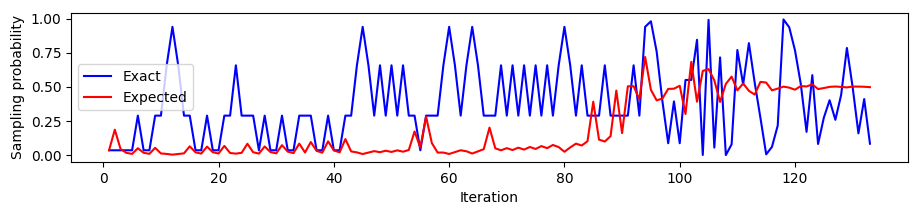
\includegraphics[width=0.8\textwidth]{exae-expected-probability}
	\caption{Exact and expected probability calculation for a single run of SAE.}
	\label{fig::exae-expected-probability}
\end{figure}

\subsubsection{Decohering Noise}
We explore the performance of our algorithm for a range of noise rates.

As shown in Figure \ref{fig::ExAE-noisy-max-depth}, the algorithm will not go beyond a depth of $\sim \frac{1}{\lambda}$.

\begin{figure}[htbp]
	\centering
	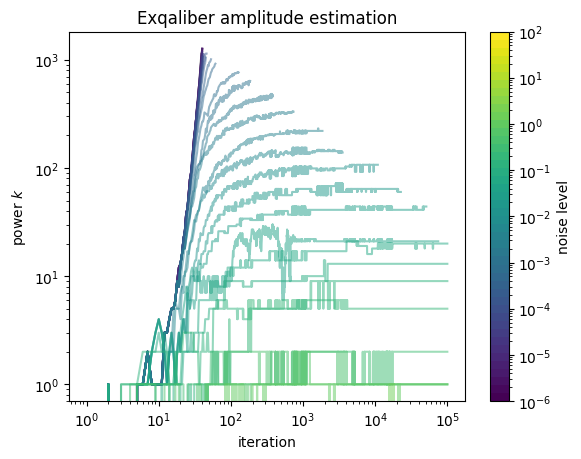
\includegraphics[scale=0.5]{ExAE-noisy-max-depth}
	\caption{Depth of SAE for $\theta_0 = 1$ at varying levels of decohering noise characterised by $\lambda = 10^0, 10^{-1}, \ldots 10^{-6}$. The prior for each iteration is taken to be $N(\pi /2, 1)$, we target $\varepsilon = 10^{-3}$ and success probability $1 - \alpha$ with $\alpha = 0.01$.}
	\label{fig::ExAE-noisy-max-depth}
\end{figure}

\begin{figure}[htbp]
	\centering
	\missingfigure{}
	\caption{Total number of oracle queries for SAE with decohering noise characterised by $\lambda = 10^{-1}, 10^{-2}, \ldots, 10^{-7}$. Each point is a single value of $\theta_0 \in \Theta_0$. We sample uniformly from $\Theta_0$ for 30 values of $\theta_0$. Each value of $\theta_0$ is evaluated for all decohering noise values and each target $\varepsilon$. The prior for each iteration is taken to be $N(\theta_0, 1)$ and success probability $1 - \alpha$ with $\alpha = 0.01$.}
	\label{fig::query-exae-noisy}
\end{figure}

\begin{itemize}
	\color{red}
	\item Concerned that error comparisons make no sense here. These algorithms have no capacity to cope with noise so obviously they're bad - but others e.g. Hitachi, QoPrime, Power-law AE do
\end{itemize}

\begin{figure}[htbp]
	\centering
	\missingfigure{}
	\caption{Final precision versus total number of oracle queries used for IAE, MLAE and SAE with decohering noise characterised by $\lambda = 10^{-3}$. We target precisions of $\varepsilon = 10^{-3}, 10^{-4}, \ldots , 10^{-7}$, with each point a single value of $\theta_0 \in \Theta_0$. We sample uniformly from $\Theta_0$ for 30 values of $\theta_0$. Each value of $\theta_0$ is evaluated for all algorithms and each target $\varepsilon$. The prior for each iteration is taken to be $N(\theta_0, 1)$ and success probability $1 - \alpha$ with $\alpha = 0.01$.}
	\label{fig::query-comparison-noisy}
\end{figure}

\newpage



%% This is probably explained earlier, but I need it for my argument, so I wrote it. In the final version, we probably need to refer to earlier in the text.
%In amplitude estimation, there is an operator $\mathcal{A}$ acting on $n+1$ qubits, such that $\mathcal{A} \ket{\psi}_{n+1} = \sqrt{a}\ket{\psi_1}_{n}\ket{1} + \sqrt{1-a}\ket{\psi_0}_n\ket{0}$,
%with $a\in [0,1]$ or, when defining $a=\sin^2{\theta_a}$ with $\theta_a \in [0, \pi]$,
%\begin{equation}
%	\mathcal{A}_{n+1} \ket{\psi} = \sin{\theta_a} \ket{\psi_1}_n \ket{1}
%	+ \cos{\theta_a}\ket{\psi_0}_n\ket{0}.
%\end{equation}
%The goal is to find $\theta_a$.
%
%One can create an operator $\mathcal{Q} = \mathcal{A} \mathcal{S}_0 \mathcal{A}^{\dagger}\mathcal{S}_{\psi_0}$ with $\mathcal{S}_{\psi_0} = \mathbb{I} - 2\ket{\psi_0}_n\bra{\psi_0}_n\otimes\ket{0}\bra{0}$ and $\mathcal{S}_0 = \mathbb{I} - 2\ket{0}_{n+1}\bra{0}_{n+1}$. % TODO reference
%% TODO choose definition of 'oracle queries'. In the iterative AE paper, they "denote applications of Q as quantum samples or oracle queries."
%Now by applying $\mathcal{Q}$ for $k$ times (and thereby applying $\mathcal{A}$ a total of $(2k+1)$ times), the probability of measuring the $\ket{1}$ state follows a Bernoulli distribution with $p$ equal to
%\begin{equation}
%	p = \frac{1}{2}(1-\cos{((2k+1)\theta_a)}).
%	\label{eq:bernoulli-p}
%\end{equation}
%Using this equation, one can test different amplitude estimation analytically, by sampling from the Bernoulli distribution directly. We call this direct analytical sampling.
%
%We experimented with our novel amplitude estimation routine. There are two relevant measures for amplitude estimation.
%These are the time to solution (and its scaling) and the quality of the solution, i.e., the error $\epsilon$.
%To measure these, we simulate experiments using direct analytical sampling.
%
%
%As our algorithm uses dynamical updates, depending on the true $\theta$, %TODO: make this consistent throughout the article. Maybe theta hat?
%anomalies can rise for values around integer fractions of $\pi$.
